\section{CI/CD Pipeline}
We maintained and extended our Gitlab CI/CD Pipeline to a three-step process. The first one builds the web application and prepares our PostgreSQL database. In the second step, we execute our backend and frontend unit tests. And lastly, we check for code smells and style with our linter.

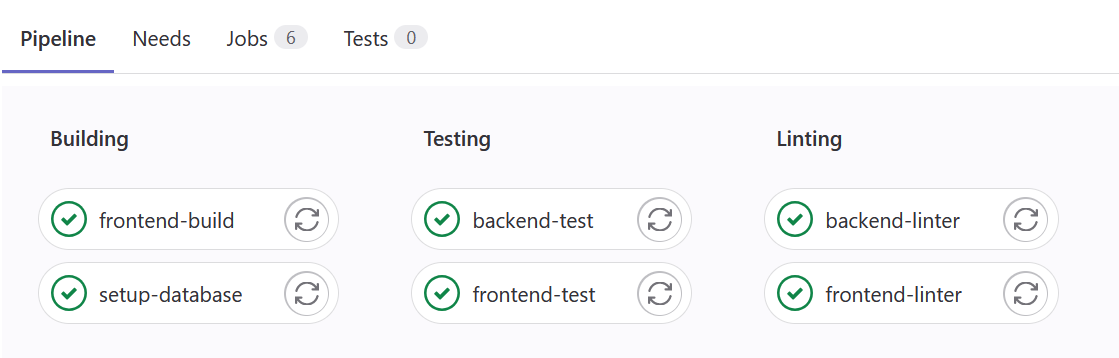
\includegraphics[width=1\textwidth]{images/pipeline.png}


This three-step process in our Gitlab CI/CD pipeline has been extremely beneficial for our testing phase.

Firstly, by building the web application and preparing the PostgreSQL database in the initial step, we ensure that all necessary dependencies are installed and the environment is properly set up. This helps us avoid any errors or issues that may arise from missing dependencies or configuration problems.

Secondly, executing backend and frontend unit tests in the second step ensures that all changes made to the codebase do not break existing functionality. The unit tests act as a safety net that helps us catch any issues or bugs before they make it to the production environment. By running the tests in an automated way through the CI/CD pipeline, we can ensure that the tests are always run consistently, and we can easily detect issues as soon as they arise.

Finally, the third step in our pipeline checks for code smells and style with our linter. This helps us maintain a high level of code quality and consistency throughout the project. By catching potential issues with code style or best practices early on, we can avoid issues and ensure that the code is easy to maintain and extend in the future.

Overall, by maintaining and extending our Gitlab CI/CD pipeline to a three-step process, we have been able to improve the quality and reliability of our web application. The pipeline provides us with a consistent and automated way to build and test our code, catch issues early on, and ensure that our codebase adheres to best practices and style guidelines.
